\documentclass[dvipdfmx,autodetect-engine,titlepage]{jsarticle}
\usepackage[dvipdfm]{graphicx}
\usepackage{ascmac}
\usepackage{fancybox}
\usepackage{listings}
\usepackage{plistings}
\usepackage{itembkbx}
\usepackage{amsmath}
\usepackage{svg}
\usepackage{url}
\usepackage{graphics}
\usepackage{listings,jvlisting}
\usepackage{scalefnt}

\textheight=23cm
\renewcommand{\figurename}{図}
\renewcommand{\tablename}{表}
\newenvironment{code}
{\vspace{0.5zw}\VerbatimEnvironment  
\begin{screen} 
\baselineskip=1.0\normalbaselineskip
 \begin{Verbatim}}
{\end{Verbatim}
\baselineskip=\normalbaselineskip
 \end{screen}\vspace{0.5zw}} 

\title{情報理工学部 SNコース 2回\\
セキュリティ・ネットワーク学実験2\\
NW実験2-1レポート}
\author{2600200443-6\\Yamashita Kyohei\\山下 恭平}
\date{November 17 2021}

\begin{document}

\maketitle

\section{実験概要}

\section{実行結果}
\begin{figure}[h]
  \centering
  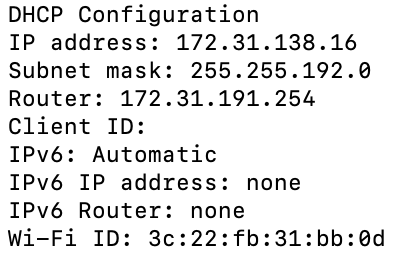
\includegraphics[scale=1]{SS1.png}
\end{figure}

\section{表示された項目とその意味}

 \subsection{DHCP Configuration}
 DHCPは「Dynamic Host Configuration Protocol」の略であり、IPv4ネットワー
 クにおいて通信用の基本的な設定を自動的に行うためのプロトコルである。このプロトコル
 はIPv4での通信を行う際に必要なIPv4アドレス、サブネットマスク、デフォルトゲート
 ウェイ、DNSサーバのIPアドレスなどが自動で設定される。\\
 DHCP Configurationであるので、この下に表示されている情報は、このプロトコルに
 よって得られたものを表示していると考えられる。

 \subsection{IP Address}
 IP Addressはネットワーク上の機器を識別するために設定される、識別用の番号である。
 IPアドレスはネットワー部とホスト部で構成されており、どの部分がそれに対応するかは
 サブネットマスクにて識別される。

 \subsection{Subnet mask}
 Subnet maskとは、IPアドレスを分割しどこがネットワークアドレス部分で、どこが
 端末を表すホスト部分かを識別するために使用する数値。

 \subsection{Router}
 ルータのIPアドレス(IPv4)


 \subsection{Client ID}
 Client IDはMQTTクライアントを識別するための23バイトのストリング。

 \subsection{IPv6}
 IPアドレスを128ビットのデータとして表現する方法。この方法であれば約340澗個(1垓の1京倍)
 のIPアドレスを割り当て可能であり、事実上無限台のコンピュータにIPアドレスを割り当てること
 ができる。

 \subsection{IPv6 IP Address}
 128ビットで表現されるIPアドレス。

 \subsection{IPv6 Router}
 ルータのIPアドレス(IPv6)

 \subsection{Wi-Fi ID}
 このコンピュータのネットワークインターフェースが持つ、固有の番号。MACアドレス、物理アドレス
 とも呼ばれ、16進数で表現される。

\section{IPアドレスの変換}
表示されているIPアドレスは「172.31.138.16」であるので、これを2進数に変換すると\\
「10101100.00011111.10001010.00010000」となる。

\section{ネットワークインターフェースのベンダーの調査}

\subsection{使用しているコンピュータのベンダー}
私が使用しているコンピュータのベンダーは「Apple,Inc.」であった。私はMacを使用しているの、当然であると考えられる。
以下の図は検索結果である。

\begin{figure}[h]
  \centering
  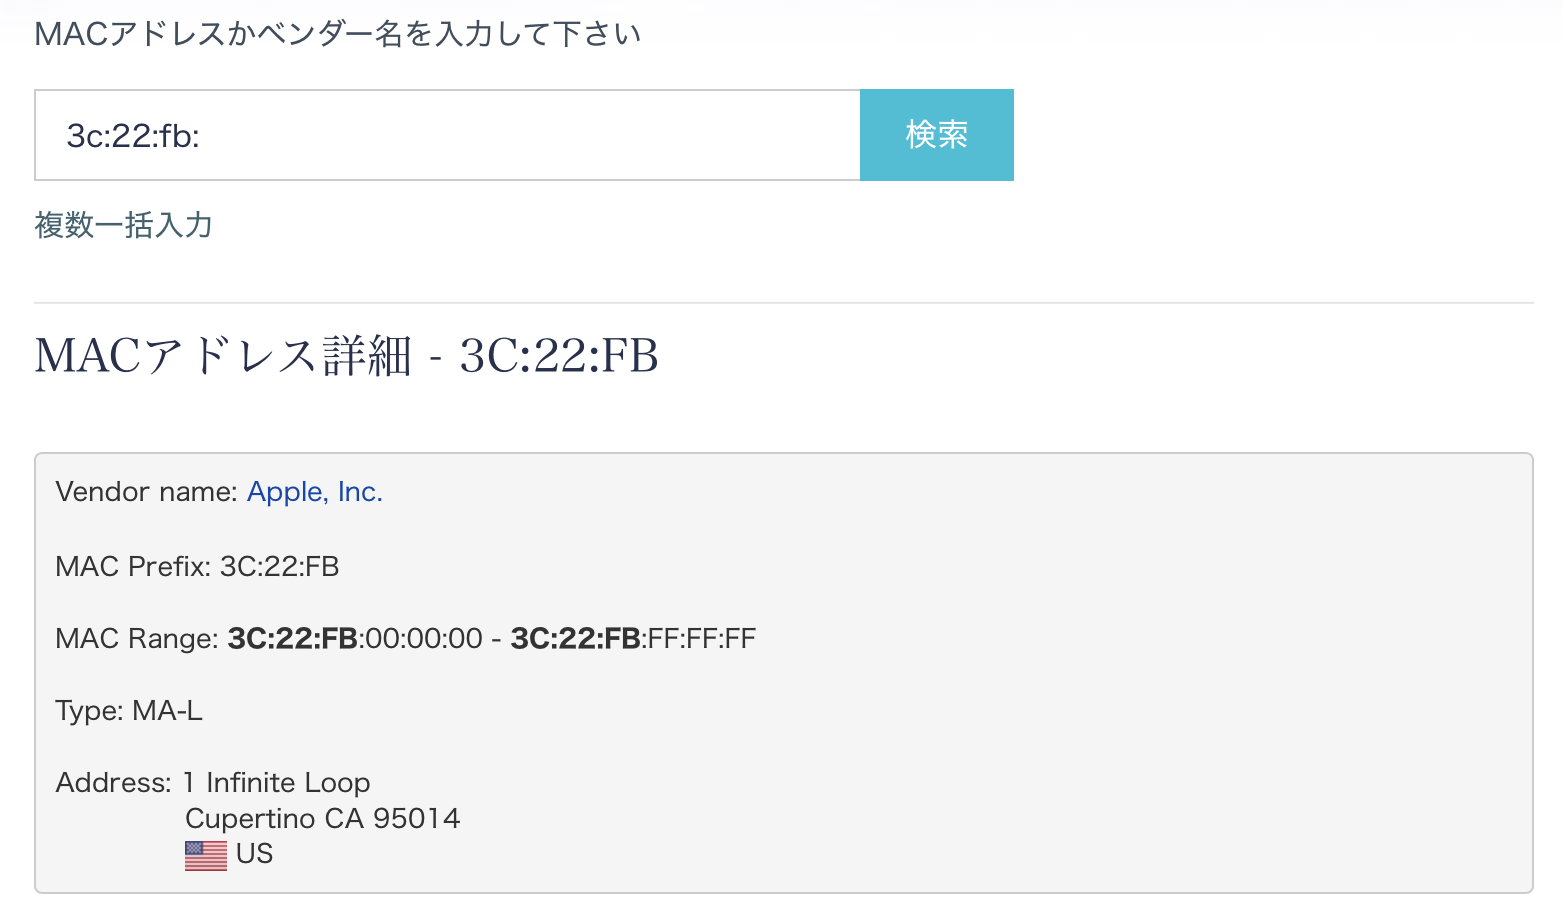
\includegraphics[scale=0.3]{SS2.png}
  \caption{検索結果}
\end{figure}

\subsection{AppleのOUI}
AppleのOUIを5つ調べて結果は以下である。\\
「00:03:93」\\「10:94:BB」\\「2C:F0:EE」\\「4C:32:75」\\「68:09:27」




\end{document}

